\section{Матричный калькулятор}

\subsection{Условие задания}

Создать приложение, реализующее основные операции с векторами и матрицами:
\begin{enumerate}
    \item Ввод матрицы, вектора
    \item Создание матриц (единичная, матрица как набор векторов)
    \item Умножение на число, вектор, матрицу
    \item Сложение/вычитание двух матриц
    \item Сложение/вычитание двух векторов
    \item Скалярное и векторное произведение двух векторов
    \item Транспонированная матрица
    \item Определитель, ранг матрицы
\end{enumerate}
Выводить сообщения об ошибках (ввод не числа, несоответствие размерностей)

\subsection{Вид формы в конструкторе}



Создано окно приложения, содержащее пять элементов TextBox, четыре элемента Label, четыре элемента Button, один элемент gridview и один элемент ErrorProvider для обработки ошибок. Вид окна представлен на рисунке \ref{task6_form} \cite{stroustrup2013c++}.
\begin{figure}[H]
    \centering
    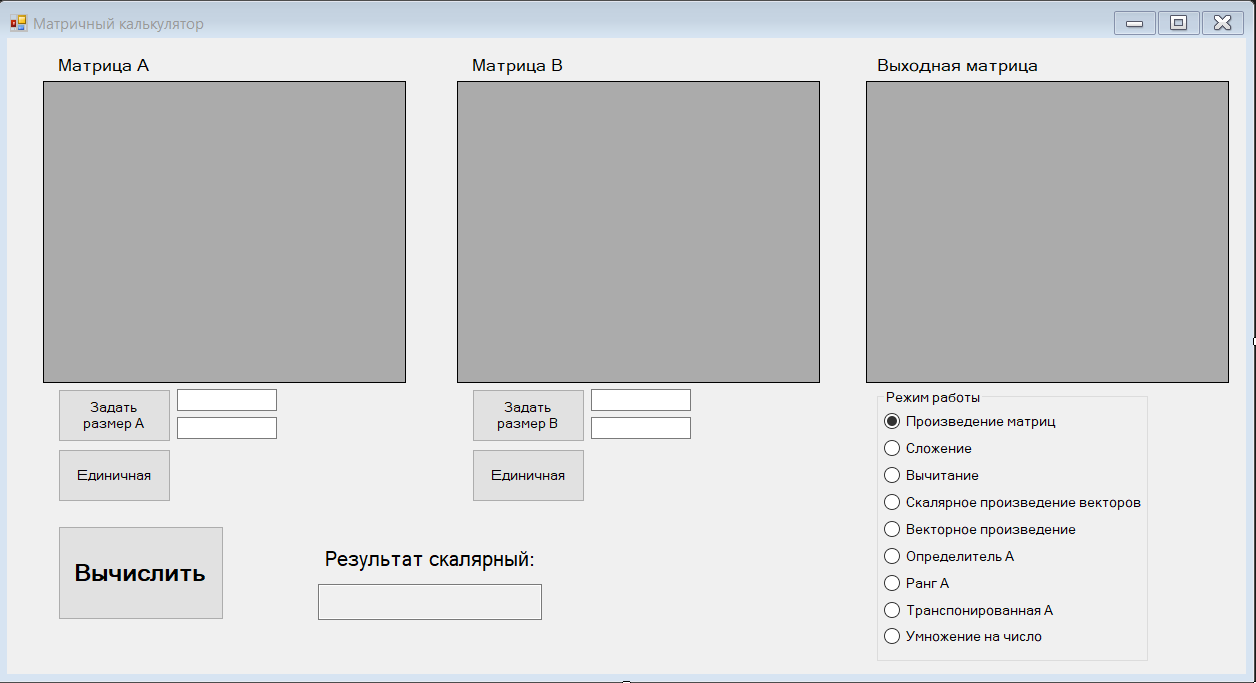
\includegraphics[width=1\linewidth]{lections/img/task6_form.png}
    \caption{Окно приложения «Матричный калькулятор» открытое в конструкторе}
    \label{task6_form}
\end{figure}

\subsection{Таблица с описанием переименованных элементов формы}
Все измененные элементы формы указаны в таблице \ref{task6_attributes}.

\begin{longtable}{|l|l|l|}
\caption{Значения атрибутов элементов в приложении <<Матричный калькулятор>>}\label{task6_attributes}\\
\hline
\textbf{\begin{tabular}[c]{@{}l@{}}Описание элементов\\ формы\end{tabular}}                   & \textbf{\begin{tabular}[c]{@{}l@{}}Список измененных\\ атрибутов\end{tabular}} & \textbf{\begin{tabular}[c]{@{}l@{}}Новое значение\\ атрибута\end{tabular}} \\ \hline
\endfirsthead
%
\endhead
%
Форма MyForm                                                                                  & Text                                                                           & Матричный калькулятор                                                      \\ \hline
\begin{tabular}[c]{@{}l@{}}TextBox ввода количества\\ строк Матрицы А\end{tabular}            & Name                                                                           & set\_size\_A\_lines                                                        \\ \hline
\begin{tabular}[c]{@{}l@{}}TextBox ввода количества\\ столбцов таблицы А\end{tabular}         & Name                                                                           & set\_size\_A\_columns                                                      \\ \hline
\begin{tabular}[c]{@{}l@{}}TextBox ввода количества\\ строк Матрицы B\end{tabular}            & Name                                                                           & set\_size\_B\_lines                                                        \\ \hline
\begin{tabular}[c]{@{}l@{}}TextBox ввода количества\\ столбцов матрицы В\end{tabular}         & Name                                                                           & set\_size\_B\_columns                                                      \\ \hline
\multirow{2}{*}{\begin{tabular}[c]{@{}l@{}}Кнопка "Единичная" под \\ матрицей А\end{tabular}} & Name                                                                           & edbtn                                                                      \\ \cline{2-3} 
                                                                                              & Text                                                                           & Единичная                                                                  \\ \hline
\multirow{2}{*}{\begin{tabular}[c]{@{}l@{}}Кнопка "Единичная" под \\ матрицей B\end{tabular}} & Name                                                                           & edbtnB                                                                     \\ \cline{2-3} 
                                                                                              & Text                                                                           & Единичная                                                                  \\ \hline
\multirow{2}{*}{Кнопка "Вычислить"}                                                           & Name                                                                           & solve                                                                      \\ \cline{2-3} 
                                                                                              & Text                                                                           & Вычислить                                                                  \\ \hline
\begin{tabular}[c]{@{}l@{}}TextBox вывода скалярного\\ ответа\end{tabular}                    & Name                                                                           & output\_scal                                                               \\ \hline
\multirow{2}{*}{Кнопка "Задать размер" А}                                                     & Name                                                                           & set\_size\_A                                                               \\ \cline{2-3} 
                                                                                              & Text                                                                           & Задать размер A                                                            \\ \hline
\multirow{2}{*}{Кнопка "Задать размер" В}                                                     & Name                                                                           & set\_size\_B                                                               \\ \cline{2-3} 
                                                                                              & Text                                                                           & Задать размер B                                                            \\ \hline
\multirow{3}{*}{Таблица Матрица А}                                                            & Name                                                                           & input\_A                                                                   \\ \cline{2-3} 
                                                                                              & AllowUserToAddRows                                                             & False                                                                      \\ \cline{2-3} 
                                                                                              & AllowUserToDeleteRows                                                          & False                                                                      \\ \hline
\multirow{3}{*}{Таблица Матрица B}                                                            & Name                                                                           & input\_B                                                                   \\ \cline{2-3} 
                                                                                              & AllowUserToAddRows                                                             & False                                                                      \\ \cline{2-3} 
                                                                                              & AllowUserToDeleteRows                                                          & False                                                                      \\ \hline
\multirow{4}{*}{Таблица выходной матрицы}                                                     & Name                                                                           & output\_grid                                                               \\ \cline{2-3} 
                                                                                              & AllowUserToAddRows                                                             & False                                                                      \\ \cline{2-3} 
                                                                                              & AllowUserToDeleteRows                                                          & False                                                                      \\ \cline{2-3} 
                                                                                              & ReadOnly                                                                       & True                                                                       \\ \hline
\multirow{2}{*}{\begin{tabular}[c]{@{}l@{}}GroupBox выбора режима\\ работы\end{tabular}}      & Name                                                                           & modes                                                                      \\ \cline{2-3} 
                                                                                              & Text                                                                           & Режим работы                                                               \\ \hline
\multirow{3}{*}{\begin{tabular}[c]{@{}l@{}}RadioButton Произведение\\ матриц\end{tabular}}    & Name                                                                           & mode1\_proiz                                                               \\ \cline{2-3} 
                                                                                              & Text                                                                           & Произведение матриц                                                        \\ \cline{2-3} 
                                                                                              & Checked                                                                        & True                                                                       \\ \hline
\multirow{2}{*}{RadioButton Сложение}                                                         & Name                                                                           & mode2\_sloz                                                                \\ \cline{2-3} 
                                                                                              & Text                                                                           & Сложение                                                                   \\ \hline
\multirow{2}{*}{RadioButton Вычитание}                                                        & Name                                                                           & mode3\_sub                                                                 \\ \cline{2-3} 
                                                                                              & Text                                                                           & Вычитание                                                                  \\ \hline
\multirow{2}{*}{\begin{tabular}[c]{@{}l@{}}RadioButton Скалярное\\ произведение\end{tabular}} & Name                                                                           & mode4\_skalproz                                                            \\ \cline{2-3} 
                                                                                              & Text                                                                           & \begin{tabular}[c]{@{}l@{}}Скалярное произведение\\ векторов\end{tabular}  \\ \hline
\multirow{2}{*}{\begin{tabular}[c]{@{}l@{}}RadioButton векторное\\ произведение\end{tabular}} & Name                                                                           & mode5\_vectproz                                                            \\ \cline{2-3} 
                                                                                              & Text                                                                           & Векторное произведение                                                     \\ \hline
\multirow{2}{*}{RadioButton Определитель А}                                                   & Name                                                                           & mode6\_oprA                                                                \\ \cline{2-3} 
                                                                                              & Text                                                                           & Определитель А                                                             \\ \hline
\multirow{2}{*}{RadioButton Ранг А}                                                           & Name                                                                           & mode7\_rankA                                                               \\ \cline{2-3} 
                                                                                              & Text                                                                           & Ранг А                                                                     \\ \hline
\multirow{2}{*}{\begin{tabular}[c]{@{}l@{}}RadioButton\\ Транспонированная А\end{tabular}}    & Name                                                                           & mode8\_tranA                                                               \\ \cline{2-3} 
                                                                                              & Text                                                                           & Транспонированная А                                                        \\ \hline
\multirow{2}{*}{\begin{tabular}[c]{@{}l@{}}RadioButton Умножение\\ на число\end{tabular}}     & Name                                                                           & mode9\_numproz                                                             \\ \cline{2-3} 
                                                                                              & Text                                                                           & Умножение на число                                                         \\ \hline
\end{longtable}


\subsection{Примеры правильной и неправильной работы}
После запуска программы на экране появляется окно на рисунке \ref{task6_launch1}.
\begin{figure}[H]
    \centering
    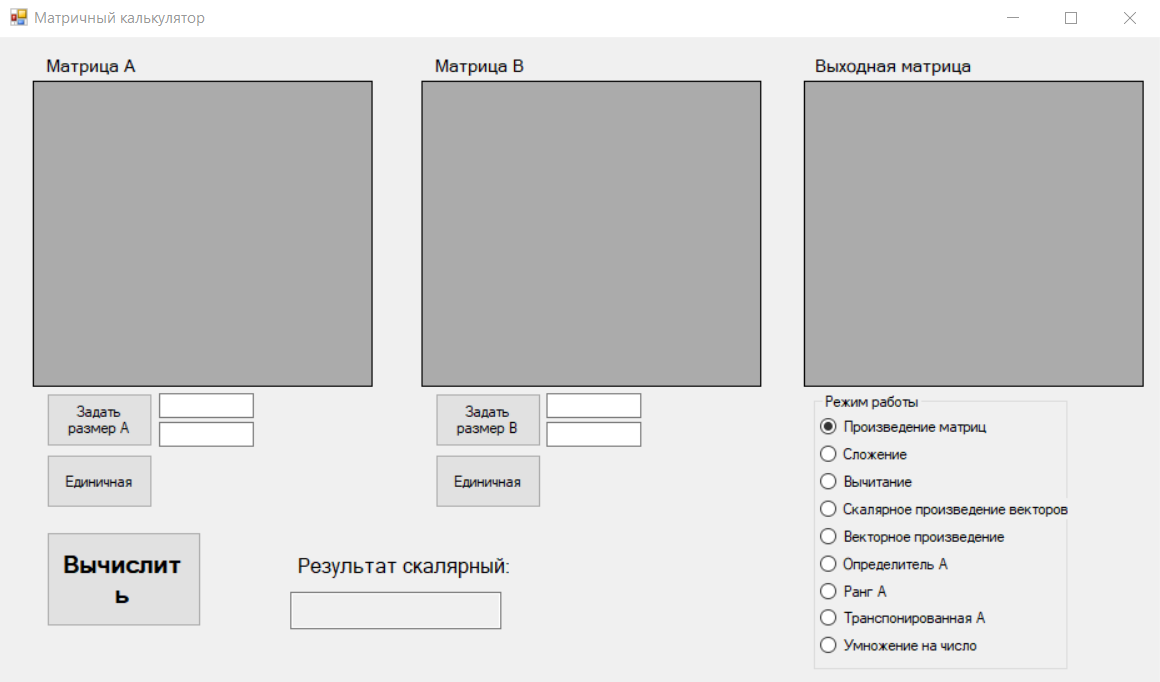
\includegraphics[width=1\linewidth]{lections/img/task6_launch1.png}
    \caption{Запуск программы}
    \label{task6_launch1}
\end{figure}

После ввода двух матриц и нажатии на кнопку "Вычислить" (на рисунке \ref{task6_launch2}).

\begin{figure}[H]
    \centering
    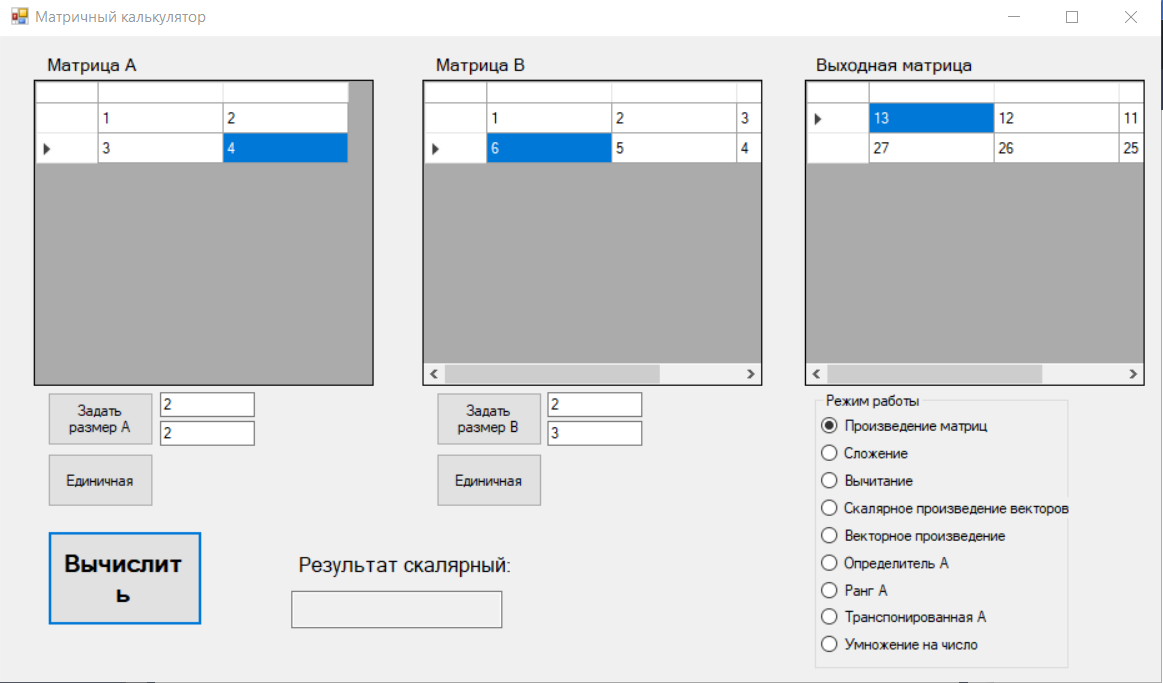
\includegraphics[width=1\linewidth]{lections/img/task6_launch2.png}
    \caption{Произведение матриц}
    \label{task6_launch2}
\end{figure}

При попытке ввода не числа в таблицу, программа выведет ошибку (на рисунке \ref{task6_launch3})
\begin{figure}[H]
    \centering
    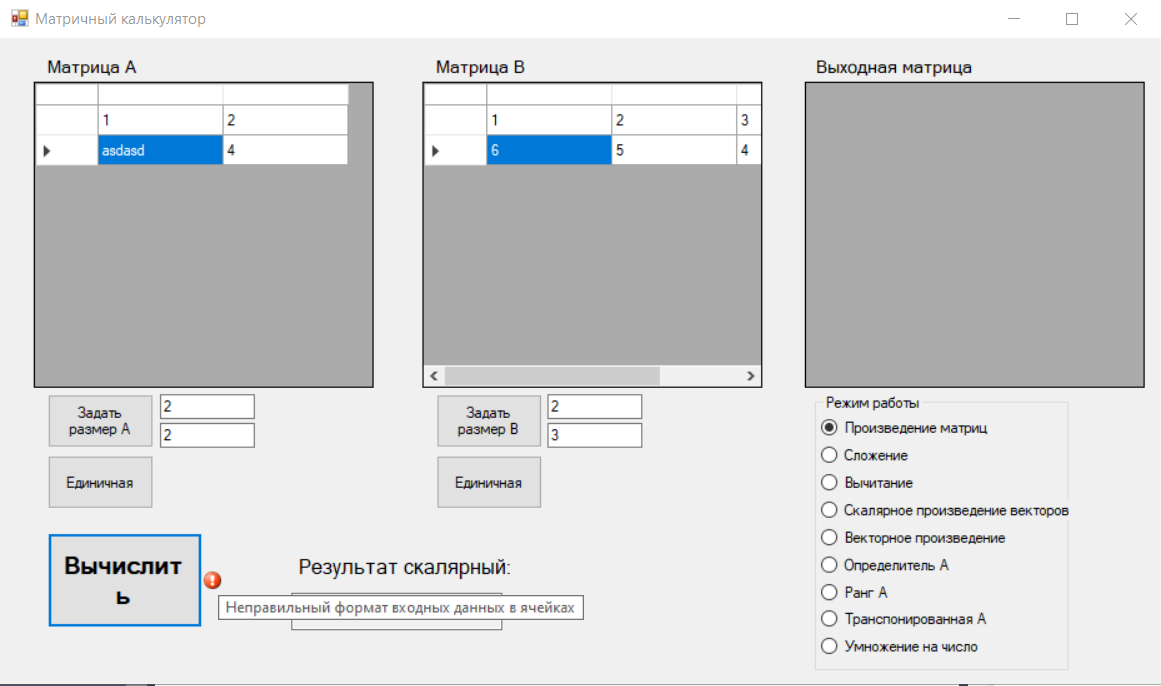
\includegraphics[width=1\linewidth]{lections/img/task6_launch3.png}
    \caption{Ошибка формата ввода}
    \label{task6_launch3}
\end{figure}


\subsection{Примеры исходного кода}


Функция cоздания единичной матрицы B.
\begin{minted}[style=bw,
 linenos=true,
 breaklines=true,
 numbersep=5pt,
 tabsize=2,
 fontsize=\small,
 bgcolor=white]{cpp}
private: System::Void edbtnB_Click(System::Object^ sender, System::EventArgs^ e) {
	int line_count = this->input_B->RowCount;
	int column_count = this->input_B->ColumnCount;
	try {
		if (line_count != column_count) throw gcnew Exception("Матрица не квадратная");
		for (int i = 0; i < line_count; i++) {
			for (int j = 0; j < line_count; j++) {
				if (i == j) this->input_B->Rows[i]->Cells[j]->Value = 1;
				else this->input_B->Rows[i]->Cells[j]->Value = 0;
			}
		}
	}
	catch (Exception^ e) {
		this->errorProvider1->SetError(this->solve, e->Message);
	}
}
\end{minted}
Другие фрагменты кода расположены в приложении \ref{app:matrix}.
\sectionbreak